% Materials and Methods
\section{Materials}
All experiments and measurements were conducted within the facilities of Systems Neuroscience and Neurotechnology Unit, particularly the Green Lab, located at the University Hospital Saarland, and the Mindscan Lab, located at the HTW Saar (Technikum).

\subsection{System Components}
% The system (in lack of a better word) is compriesed of a variety of different components, be it commercial hardware used in the final system or the experiment setup, or software that has been created in the scope of the present thesis. Therefore, this subsection is dedicated to the above mentioned components, especially those originating in the process of this work.
\subsection{Hardware}
\textbf{Empatica E4 Wristband}
The Empatica E4 wristband is a wearable wireless device designed for comfortable, continuous, real-time data acquisition. It is a class IIa medical device in the EU, according to CE Cert. No. 1876/MDD (93/42/EEC Directive) and was designed for daily life usage \cite{e4}.

%\begin{figure}[ht]
%	\centering
%  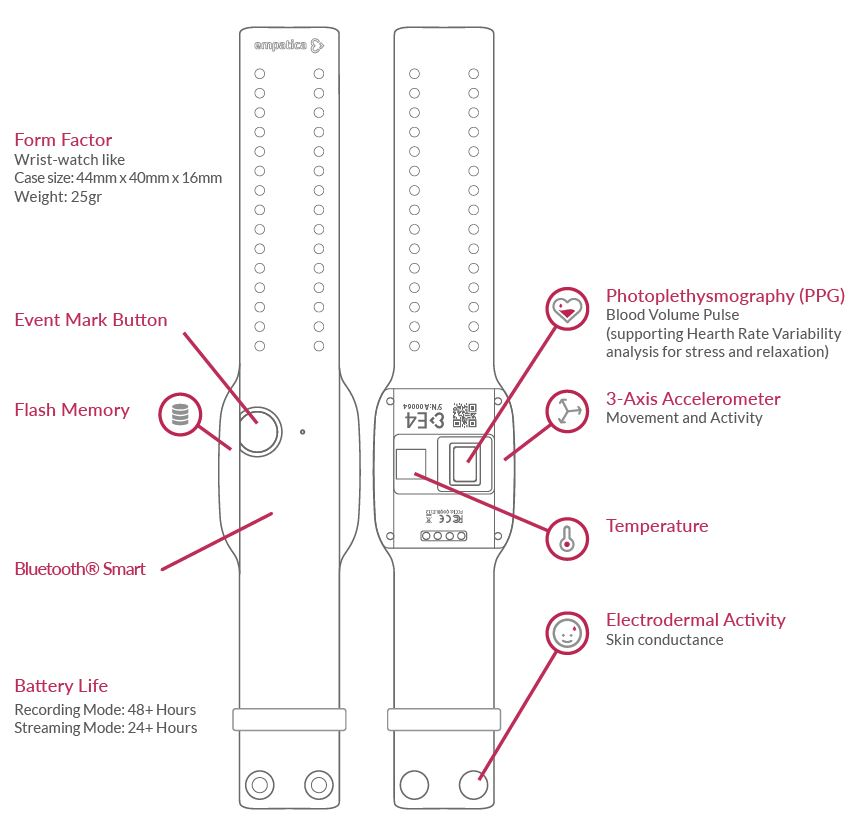
\includegraphics[width=0.33\textwidth]{../images/E4overview.JPG}
%	\caption{Overview of the Empatica E4 wristband.}
%	\label{e4overview}
%\end{figure}

Figure \ref{e4overview} shows an overview of the entire E4 wristband from either side indicating key attributes as wells as a total of four different sensors that will be discussed briefly in the following:

\begin{itemize}
\item \textbf{Photoplethysmography (\gls{ppb})} to provide blood volume pulse (\gls{bvp}), from which heart rate, heart rate variability and other cardiovascular features may be derived
\item \textbf{Electrodermal activity (\gls{eda})} is used to measure sympathetic nervous system arousal and to derive features related to stress, engagement and excitement
\item \textbf{3-Axis accelerometer} to capture motion-based activity
\item \textbf{Infrared thermopile} for reading skin temperature
\end{itemize}

As the E4 is intended to be worn on the wrist these sensors are set up in a specific way to provide for optimal use. As can be seen on \ref{e4overview} the majority of the sensors are located on the backside of the main unit not including the \gls{eda}-sensor, which is located on the wristband itself. 

Wearing the E4 wristband is equally intrusive to wearing a watch and therefore providing a high level of convenience compared to other physiologic measures such as electrocardiogram \gls{ecg} or electroencephalogram \gls{eeg}.

\textbf{Sampling Specifications}
All recordings were performed using only software licensed by Empatica. Using the approved streaming application and the compatible Bluetooth receiver, the recorded data was streamed directly to an operator's personal computer via a Bluetooth connection. 

\textbf{EDA sensor}
\begin{itemize}
\item Sampling frequency: 4 Hz (Non customizable).
\item Resolution: 1 digit ~900 pSiemens.
\item Range: 0.01 $\mu$Siemens – 100 $\mu$Siemens.
\item Alternating current (8Hz frequency) with a
max peak to peak value of 100 $\mu$Amps (at 100
$\mu$Siemens).
\item Electrode(Placement): on the ventral (inner) wrist.
\item Electrode(Build): Snap-on, silver (Ag) plated with metallic core.
\item Electrode(Longevity): 4–6 months
\end{itemize}

\textbf{PPG sensor}
\begin{itemize}
\item Sampling frequency 64 Hz (Non customizable).
\item LEDs: Green (2 LEDs), Red (2 LEDs) Photodiodes: 2
units, total 15.5 mm2 sensitive area.
\item Sensor output: Blood Volume Pulse (BVP) (variation
of volume of arterial blood under the skin resulting
from the heart cycle).
\item Sensor output resolution 0.9 nW / Digit.
\item Motion artifact removal algorithm: Combines different light wavelengths. Tolerates external lighting conditions.
\end{itemize}

\textbf{Infrared Thermopile}
\begin{itemize}
\item Sampling frequency: 4 Hz (Non customizable).
\item Range(Ambient temperature): -40...85$\deg$C (if available).
\item Range(Skin temperature): -40...115$\deg$C.
\item Resolution: 0.02$\deg$C.
\item Accuracy $\pm$0.2$\deg$C within 36-39$\deg$C.
\end{itemize}

\textbf{Real-time clock}
\begin{itemize}
\item Resolution(Recording mode): 5s synchronization resolution. Average of 6 seconds in 6 million seconds drift.
\item Resolution(Streaming mode): Temporal resolution up to 0.2 seconds with connected device.
\end{itemize}

\section{Methods}
\subsection{Experiment}
\textbf{Participants}
% talk about composition of subject group

\textbf{Paradigm}
One of the most important parts to this project was the collection of authentic data that could be used later on to develop a reliable classifier for our system. For that reason a experiment, specifically designed to elicit certain emotional and cognitive states in a subject, was conducted. The following section is focused on the procedure applied in this experiment.

The procedure was comprised of a total of five sessions. Every experiment was initiated with a short briefing session. Containing a short questionnaire, covering personal information of the participant as well as habits that may have a influence on the measurement. Further a series of questions, regarding their handedness, use and frequency of use of watches or other wearables was posed, to estimate the additional influence that may be caused by wearing the Empatica E4 wristband.
Concluding the first session, the participants were given a coarse outline of the experiment covering the structure and a basic description of their responsibilities.

The second session consisted of a baseline measurement used to log the participants form of the day and also to be able to account for environmental influences in the following processing steps. Before the start of the measurement the subject was placed on a chair in front of a monitor (24 inches, Resolution: 1080p) with a approximated distance of 1m. The Empatica E4 was then put on the wrist of the non-dominant hand and secured in a position that caused minimal light leakage to the PPG-sensor and provided optimal contact for the \gls{eda} electrodes. After the participants were comfortable with the device a one minute test sequence was measured to verify the functionality of the system.
Consequently the paradigm was displayed on the monitor and the session was started. After reading the instructions, in which the subjects were asked to relax and remain still, and confirmation with the participant the measurement was initiated with a ten second countdown to give some additional time for preparation.
During the measurement the \gls{eda}, \gls{bvp}, and temperature of the subject were measured for a duration of five minutes.
Afterwards, to conclude the second session, the participants had to give a subjective rating of their current mental state, regarding their stress level, ranging from 1 (completely relaxed) to 10 (stressed out).

The third session was comprised of three separate measurements, two cognitive tasks and a relaxation segment. As before a rating followed the recording. The ratings consisted of a subjective assessment by the subjects regarding their stress level. Additionally subjects had to rate the test difficulty on a scale from 1 (very easy) to 10 (very difficult) for both tasks. 
For the first measurement the subjects were instructed to count down aloud from 700 in steps of 7 while maintaining a certain pace. The counting rhythm was indicated by a flashing dot on the instruction screen, for a duration of five minutes. The dot's color and flashing frequency were altered during the experiment to further increase difficulty at the three and four minute mark. If the participants were to slow down or loose track an instructor would intervene to help.
The second task consisted of a Stroop-Word-Color test. The test featured 11 different colors, resulting in a total of 220 trials the subjects had to work through. Although the color palette seems rather extensive when compared to the standard 3 color variation of the test, this was a conscious decision to guarantee a test time of at least 5 minutes to mitigate monotony. Each trial presented the subject with a colored word in the center of the screen and one possible answer to either side. The participants then had to choose the right answer based on the color of the word.Each decision was recorded via a key press on the keyboard. 

%Wearing the device is as easy as wearing a watch.
%Wear the E4 with the case on top of your wrist. Wear it snugly, so that it does not move around,
%but not so tight that it is uncomfortable.
%Which side should you wear it on? Traditional recommendations are to record EDA on the nondominant
%side to minimize motion artifacts (e.g. a right-hander would wear it on their left wrist).
%However, recent studies show that the dominant side may have a much stronger EDA signal during
%certain kinds of stress. Also, neurological events (such as seizures) may elicit EDA on only one side.
%(For more information see: Picard, R. W., Fedor, S., & Ayzenberg Y., “Multiple Arousal Theory and Daily-
%Life Electrodermal Activity Asymmetry” Emotion Review, March 2015.). Depending on your purposes,
%you may want to measure on the right, left, or both wrists.
%The E4 button may be positioned on the same side as the thumb or on the other side – either
%orientation works fine.
%The EDA electrodes (under the snaps) should be on the inside of the wrist. You may optionally line
%them up with a finger, e.g. the third (ring) finger, but this is not required
%\begin{figure}[ht]
%	\centering
%  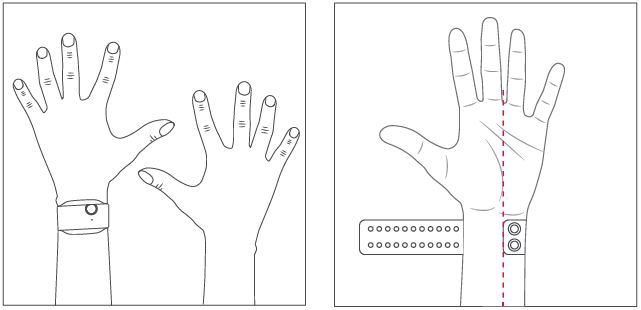
\includegraphics[width=0.33\textwidth]{../images/E4wearing.JPG}
%	\caption{A figure depicting the intended way the E4 wristband should be worn.}
%	\label{e4wearing}
%\end{figure}

\section{Signal Analysis}




\subsection{Heart Rate Variability}
% BVP PRE PROCESSING
% 	- PEAK DETECTION
%		- bandpass zero phase filtering
%		- clipping
%		- squaring
%		- moving averages
%		- thresholding
%		- blocks of interest
%		- peak detection
%		- peak validation
% INTER BEAT INTERVALS
%	- DETECT OUTLIER
%	- DETECT ECTOPIC BEATS
%	- ARTIFACT DECLARATION
%	- LINEAR INTERPOLATION
% DATA VALIDATION
% FEATURE EXTRACTION
% CLASSIFICATION AND EVALUATION

\subsection{GSR}
% GSR PRE PROCESSING
%	- low pass zero phase filtering
%	- smoothing: moving average filtering
% FEATURE EXTRACTION

\subsection{Temperature}
% TEMPERATURE PRE PROCESSING
%	- smoothing: moving average filtering
% FEATURE EXTRACTION